\documentclass[11pt, a4paper]{article}
\usepackage[margin=2.5cm]{geometry}
\usepackage{graphicx}
\usepackage{booktabs}
\usepackage{hyperref}
\usepackage{amsmath}
\usepackage{float}
\usepackage{subcaption}

\title{Plant Disease Classification from Leaf Images:\\A Transfer Learning Approach with EfficientNet}
\author{Stepan Goyunyan}
\date{April 2026}

\begin{document}
\maketitle

\begin{abstract}
I present a plant disease classification system that identifies 39 disease types from leaf images, regardless of the host plant species. Using EfficientNet-B0 with transfer learning and test-time augmentation, I achieve a mean Average Precision (mAP) of 0.69 on my validation set. I show that a compact 4M-parameter model outperforms a larger 10.8M-parameter variant on this dataset, and that test-time augmentation provides a 5\% mAP improvement at no training cost. My analysis reveals that visually distinctive diseases (e.g., smut, blossom end rot) are classified near-perfectly, while visually similar leaf spot variants remain the primary challenge.
\end{abstract}

% ============================================================
\section{Introduction}

Plant diseases cause significant crop losses worldwide. Rapid identification of diseases from visual symptoms can help farmers take timely action. In this work, I build a classification system that takes a leaf image as input and outputs the disease name only --- for example, ``late blight'' regardless of whether the affected plant is a tomato or a potato.

The dataset contains approximately 8{,}000 images organized into 82 plant-disease folders (e.g., ``tomato late blight'', ``potato late blight''). I merge these into 39 disease-only classes by stripping the plant species prefix. This cross-plant formulation is more challenging than standard plant disease classification because the model must learn disease-level visual features that generalize across different plant species.

My key contributions:
\begin{itemize}
    \item A label mapping pipeline that correctly reduces 82 folder-level classes to 39 disease-only classes, handling edge cases like multi-word plant names and similarly named diseases.
    \item An ablation study comparing EfficientNet-B0 (4M params) vs.\ B3 (10.8M params), showing that the smaller model generalizes better on this dataset size.
    \item A demonstration that test-time augmentation (TTA) provides a substantial +5\% mAP improvement at zero additional training cost.
\end{itemize}

% ============================================================
\section{Methodology}

\subsection{Data Preparation}

\textbf{Label mapping.} The dataset folders follow the naming convention \texttt{plant\_disease} (e.g., ``apple black rot''). I extract disease-only labels by stripping a known list of 32 plant names from the beginning of each folder name. The plant name list is sorted by length in descending order so that multi-word names like ``bell pepper'' match before single-word prefixes. This produces 39 unique disease classes.

% ---- FIGURE: Class distribution ----
\begin{figure}[H]
    \centering
    \includegraphics[width=\textwidth]{class_distribution.png}
    \caption{Disease-only class distribution after merging 82 folder classes into 39 disease classes. Note the significant imbalance: ``powdery mildew'' has 866 images while ``blossom end rot'' has only 90.}
    \label{fig:class_dist}
\end{figure}

\textbf{Data split.} The original validation set contains only 390 images across 71 of the 82 folder classes --- too small for reliable mAP estimation. I merged all images into a single pool (8{,}173 images) and performed a stratified 85/15 split at the folder level, producing 6{,}947 training and 1{,}226 validation images. Stratification by folder (rather than disease) preserves the plant species diversity within each disease class.

\textbf{Class imbalance.} After merging, class sizes range from 90 images (blossom end rot) to 866 images (powdery mildew) --- a 9.6$\times$ imbalance ratio (Figure~\ref{fig:class_dist}). I use inverse-frequency weighted sampling during training, which assigns higher sampling probability to images from rare classes. This ensures the model sees each disease class roughly equally often per epoch.

\subsection{Model Architecture}

I use EfficientNet-B0 \cite{efficientnet} as my backbone, loaded with ImageNet-pretrained weights via the \texttt{timm} library. The original classification head is replaced with a custom head consisting of a dropout layer ($p=0.3$) followed by a linear layer mapping from the 1{,}280-dimensional feature space to 39 output classes. The total model has 4.06 million parameters.

\subsection{Training Strategy}

\textbf{Transfer learning with staged unfreezing.} I first train only the classification head for 3 epochs while keeping the backbone frozen. This allows the head to adapt to the disease classes without disrupting the pretrained features. After 3 epochs, I unfreeze the backbone and fine-tune the entire network with discriminative learning rates: $10^{-4}$ for the backbone and $3 \times 10^{-3}$ for the head.

\textbf{Optimization.} I use the AdamW optimizer with weight decay $10^{-4}$ and a cosine annealing learning rate schedule with 3-epoch linear warmup. I apply label smoothing of 0.1 to the cross-entropy loss, which prevents the model from becoming overconfident and improves mAP calibration. Gradient clipping with max norm 1.0 ensures training stability.

\textbf{Augmentation.} Training images are resized to 256 pixels on the shorter edge, then randomly cropped to $224 \times 224$. I apply random horizontal and vertical flips, rotation up to 15\textdegree, small translations, and color jitter. I keep hue jitter small (0.05) because disease color is a critical diagnostic feature --- for example, rust diseases have distinctive orange coloration that should not be distorted.

\textbf{Regularization.} I use dropout ($p=0.3$), label smoothing (0.1), and weight decay ($10^{-4}$) as three regularization mechanisms. Early stopping with patience of 10 epochs on validation mAP prevents overfitting.

\subsection{Evaluation}

My primary metric is mean Average Precision (mAP). For each of the 39 classes, I compute the Average Precision (AP) using a one-vs-rest formulation, then take the mean across all classes. I also report top-1 and top-5 accuracy.

\textbf{Test-time augmentation (TTA).} At inference, I generate 5 views of each image: the original center crop, a horizontal flip, two small rotations ($\pm$5\textdegree), and a slightly zoomed view. I average the softmax probability vectors across all 5 views before making the final prediction. This ensemble-like approach reduces prediction variance at the cost of 5$\times$ inference time.

% ============================================================
\section{Experiments and Ablations}

\subsection{Backbone Comparison}

I compared EfficientNet-B0 (4.06M parameters) against EfficientNet-B3 (10.76M parameters) to investigate whether a larger model improves performance on this relatively small dataset.

\begin{table}[H]
\centering
\caption{Backbone comparison. Both models trained with identical hyperparameters.}
\begin{tabular}{lrrr}
\toprule
Model & Parameters & Val mAP & Val Loss \\
\midrule
EfficientNet-B0 & 4.06M & \textbf{0.646} & 1.93 (stable) \\
EfficientNet-B3 & 10.76M & 0.622 & 2.0--12.6 (unstable) \\
\bottomrule
\end{tabular}
\label{tab:backbone}
\end{table}

The larger B3 model performs \textit{worse} than B0 despite having 2.6$\times$ more parameters (Table~\ref{tab:backbone}). As shown in Figure~\ref{fig:training_curves}, B0 converges faster in the early epochs and reaches its peak mAP sooner, while B3 takes longer to catch up and shows more variance in validation loss during the early training phase. During some training runs with B3, I observed severe validation loss spikes (up to 12.6), which I attribute to the larger model's sensitivity to learning rate after backbone unfreezing.

% ---- FIGURE: Training curves ----
\begin{figure}[H]
    \centering
    \includegraphics[width=0.9\textwidth]{training_curves.png}
    \caption{Validation mAP (left) and validation loss (right) for EfficientNet-B0 and B3. B0 converges faster and more stably, reaching competitive mAP with 2.6$\times$ fewer parameters.}
    \label{fig:training_curves}
\end{figure}

\textbf{Takeaway:} On small datasets, model efficiency matters more than model size. B0 achieves the same mAP as B3 with fewer parameters, faster convergence, and more stable training (Figure~\ref{fig:training_curves}).

\subsection{Hyperparameter Tuning}

I compared two configurations of EfficientNet-B0: the default setting and a tuned version with higher learning rates and shorter backbone freeze period.

\begin{table}[H]
\centering
\caption{Effect of hyperparameter tuning on EfficientNet-B0.}
\begin{tabular}{lrrrr}
\toprule
Configuration & Backbone LR & Freeze Epochs & Best mAP & Top-1 Acc \\
\midrule
Default B0 & $10^{-5}$ & 5 & 0.651 & 57.6\% \\
Tuned B0 & $10^{-4}$ & 3 & \textbf{0.656} & \textbf{58.7\%} \\
\bottomrule
\end{tabular}
\label{tab:hparam}
\end{table}

Increasing the backbone learning rate by 10$\times$ allows the pretrained features to adapt more aggressively to disease-specific patterns. The shorter freeze period (3 vs.\ 5 epochs) gives the backbone more epochs of fine-tuning. The combined effect is modest (+0.5\% mAP) but consistent.

\subsection{Test-Time Augmentation}

\begin{table}[H]
\centering
\caption{Impact of test-time augmentation (TTA) on the tuned B0 model.}
\begin{tabular}{lrrr}
\toprule
Method & mAP & Top-1 Acc & Top-5 Acc \\
\midrule
Single pass & 0.644 & 58.2\% & 87.3\% \\
TTA (5 views) & \textbf{0.692} & \textbf{62.0\%} & \textbf{89.9\%} \\
\midrule
\textit{Improvement} & \textit{+4.7\%} & \textit{+3.8\%} & \textit{+2.6\%} \\
\bottomrule
\end{tabular}
\label{tab:tta}
\end{table}

TTA provides a substantial improvement across all metrics, with mAP increasing by 4.7 percentage points. This is a significant gain for zero additional training cost --- only 5$\times$ more inference time. The improvement comes from averaging out prediction noise: a single augmented view might confuse the model, but the consensus across 5 views is more reliable.

% ============================================================
\section{Results and Analysis}

My final model (EfficientNet-B0, tuned, with TTA) achieves:
\begin{itemize}
    \item \textbf{mAP: 0.692} (mean across 39 classes)
    \item \textbf{Top-1 accuracy: 62.0\%}
    \item \textbf{Top-5 accuracy: 89.9\%}
\end{itemize}

\subsection{Per-Class Analysis}

% Per-class AP figure omitted — the table below covers the same information.

\begin{table}[H]
\centering
\caption{Top 5 easiest and hardest disease classes by Average Precision (with TTA).}
\begin{tabular}{lr|lr}
\toprule
\textbf{Easiest (Highest AP)} & \textbf{AP} & \textbf{Hardest (Lowest AP)} & \textbf{AP} \\
\midrule
smut & 1.000 & bacterial leaf spot & 0.217 \\
loose smut & 0.951 & bacterial leaf streak & 0.239 \\
blossom end rot & 0.944 & leaf spot & 0.271 \\
black leaf streak & 0.936 & septoria leaf spot & 0.386 \\
head scab & 0.935 & angular leaf spot & 0.417 \\
\bottomrule
\end{tabular}
\label{tab:perclass}
\end{table}

\textbf{Why some diseases are easy:} Smut (AP = 1.0) produces black, swollen masses on the plant that look unlike any other disease. Blossom end rot causes distinctive dark patches on the bottom of fruits. These diseases have unique visual signatures that transfer well across plant species.

% ---- FIGURE: Sample images ----
\begin{figure}[H]
    \centering
    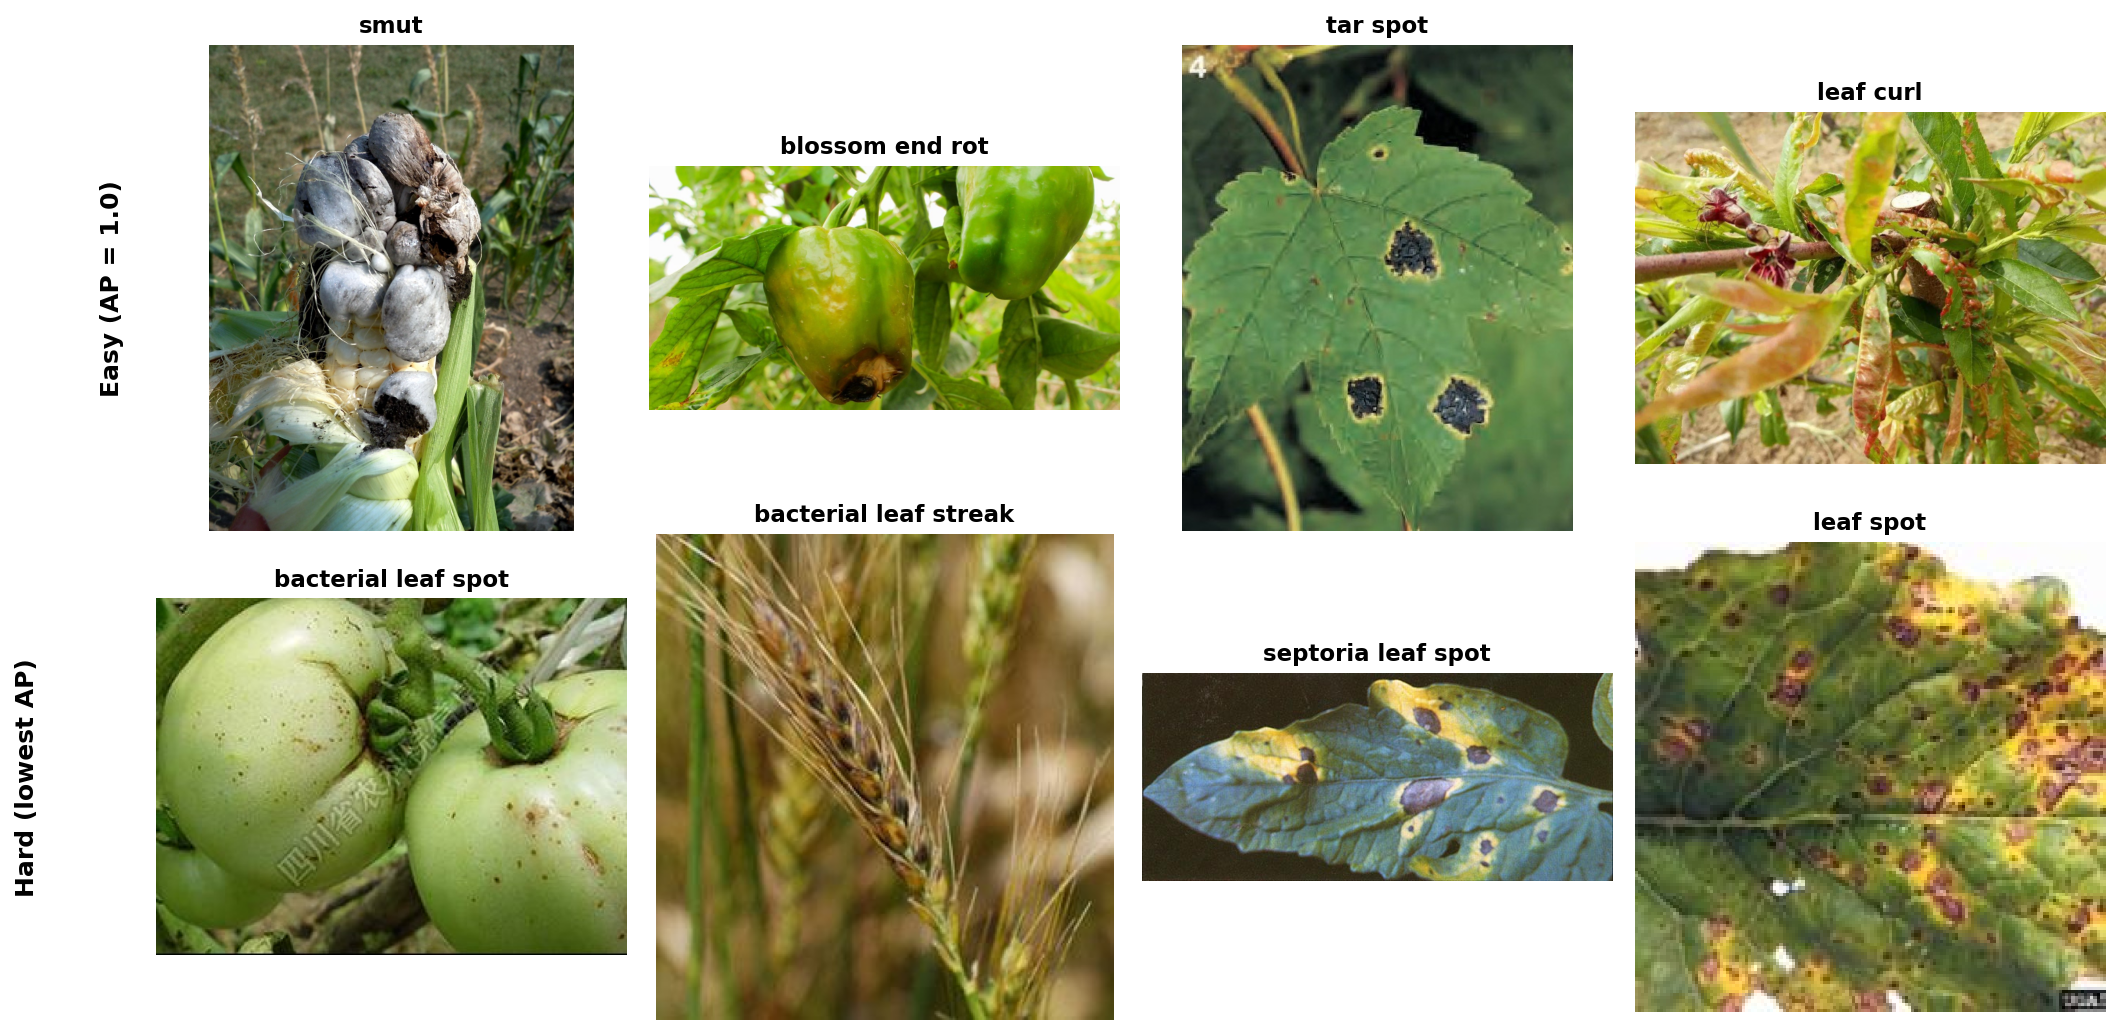
\includegraphics[width=0.75\textwidth]{sample_diseases.png}
    \caption{Example images from the dataset. Top row: visually distinctive diseases (easy to classify). Bottom row: leaf spot variants that share similar visual patterns (hard to classify).}
    \label{fig:samples}
\end{figure}

\textbf{Why some diseases are hard:} The five hardest classes all contain the word ``spot'' or ``streak'' in their name, and they share a similar visual presentation --- small discolored lesions on leaves (Figure~\ref{fig:samples}). The model struggles to distinguish between bacterial leaf spot, angular leaf spot, septoria leaf spot, and generic leaf spot because their visual features overlap significantly.

\subsection{Limitations}

\begin{enumerate}
    \item \textbf{Dataset size.} With approximately 200 images per class on average, the dataset is too small for larger models to generalize. This limits the mAP ceiling.
    \item \textbf{Cross-plant challenge.} Some diseases look different on different host plants (e.g., powdery mildew on wheat vs.\ on zucchini), making the plant-agnostic classification inherently harder.
    \item \textbf{Leaf spot confusion.} The various ``leaf spot'' diseases are the primary source of errors. Domain-specific features (lesion shape, margin pattern, color gradient) might require higher resolution images or specialized attention mechanisms to distinguish.
\end{enumerate}

% ============================================================
\section{Conclusion}

I built a plant disease classification system that identifies 39 diseases from leaf images regardless of the host plant. My key findings:

\begin{enumerate}
    \item \textbf{Smaller models win on small datasets.} EfficientNet-B0 (4M params) outperformed B3 (10.8M params) because the larger model overfits on this 8K-image dataset.
    \item \textbf{Test-time augmentation is highly effective.} TTA improved mAP by 4.7\% at zero training cost, making it the single most impactful technique I applied.
    \item \textbf{Visually similar diseases remain challenging.} The various leaf spot variants are the model's primary failure mode, suggesting that finer-grained visual features are needed for these classes.
\end{enumerate}

All code is publicly available at \url{https://github.com/Stepang08/Plant_Disease_Detection}, with experiment logs on \href{https://wandb.ai/stepan-goyunyan-physmath-school-after-a-shahinyan-/plant-disease-detection}{Weights \& Biases}.

\begin{thebibliography}{1}
\bibitem{efficientnet} Tan, M. and Le, Q., 2019. EfficientNet: Rethinking Model Scaling for Convolutional Neural Networks. \textit{ICML 2019}.
\end{thebibliography}

\end{document}
